%%%%%%%%%%%%%%%%%%%%%%%%%%%%%%%%%%%%%%%%%
% Beamer Presentation
% LaTeX Template
% Version 1.0 (10/11/12)
%
% This template has been downloaded from:
% http://www.LaTeXTemplates.com
%
% License:
% CC BY-NC-SA 3.0 (http://creativecommons.org/licenses/by-nc-sa/3.0/)
%
%%%%%%%%%%%%%%%%%%%%%%%%%%%%%%%%%%%%%%%%%

%------------------------------------------------------------------------------------------------
% PACKAGES AND THEMES
%------------------------------------------------------------------------------------------------

\documentclass[table, xcolor = {dvipsnames}, 9pt]{beamer}
\usepackage{tikz}
\usetikzlibrary{calc}
\usetikzlibrary{positioning}
\usetikzlibrary{arrows.meta}
\usetikzlibrary{external}
\mode<presentation> {

% The Beamer class comes with a number of default slide themes
% which change the colors and layouts of slides. Below this is a list
% of all the themes, uncomment each in turn to see what they look like.

\usetheme{default}
%\usetheme{AnnArbor}
%\usetheme{Antibes}
%\usetheme{Bergen}
%\usetheme{Berkeley}
%\usetheme{Berlin}
%\usetheme{Boadilla}
%\usetheme{CambridgeUS}
%\usetheme{Copenhagen}
%\usetheme{Darmstadt}
%\usetheme{Dresden}
%\usetheme{Frankfurt}
%\usetheme{Goettingen}
%\usetheme{Hannover}
%\usetheme{Ilmenau}
%\usetheme{JuanLesPins}
%\usetheme{Luebeck}
%\usetheme{Madrid}
\usetheme{metropolis}
%\usetheme{Malmoe}
%\usetheme{Marburg}
%\usetheme{Montpellier}
%\usetheme{PaloAlto}
%\usetheme{Pittsburgh}
%\usetheme{Rochester}
%\usetheme{Singapore}
%\usetheme{Szeged}
%\usetheme{Warsaw}

% As well as themes, the Beamer class has a number of color themes
% for any slide theme. Uncomment each of these in turn to see how it
% changes the colors of your current slide theme.

%\usecolortheme{albatross}
%\usecolortheme{beaver}
%\usecolortheme{beetle}
%\usecolortheme{crane}
%\usecolortheme{dolphin}
%\usecolortheme{dove}
%\usecolortheme{fly}
%\usecolortheme{lily}
%\usecolortheme{orchid}
%\usecolortheme{rose}
\usecolortheme{seagull}
%\usecolortheme{seahorse}
%\usecolortheme{whale}
%\usecolortheme{wolverine}
\usefonttheme{professionalfonts}
%\setbeamertemplate{footline} % To remove the footer line in all slides uncomment this line
%\setbeamertemplate{footline}[page number] % To replace the footer line in all slides with a simple slide count uncomment this line

%\setbeamertemplate{navigation symbols}{} % To remove the navigation symbols from the bottom of all slides uncomment this line
}

\usepackage{graphicx} % Allows including images
\usepackage{booktabs} % Allows the use of \toprule, \midrule and \bottomrule in tables
\usepackage{tikz}
\usepackage{multirow}
\usepackage{natbib}
\usepackage{hyperref}
\usepackage{diagbox}
\usepackage{makecell}
\usepackage{xparse}
\usepackage{subfig}
\usepackage{amsmath}
\usepackage{amsfonts,amsthm,amsmath,amssymb}    
\usepackage{bbm}
\usepackage{bm}
\usepackage{empheq}
\usepackage{pgfplots}
\usepackage{animate}
\usepgfplotslibrary{colorbrewer}

\newcommand\mybox[2][]{\tikz[overlay]\node[fill=lightgray,inner sep=2pt, anchor=text, rectangle, rounded corners=1mm,#1] {#2};\phantom{#2}}
\hypersetup{unicode=true,
            bookmarksnumbered=true,
            bookmarksopen=true,
            bookmarksopenlevel=2,
            breaklinks=false,
            pdfborder={0 0 1},
            hypertexnames=false,
            pdfstartview={XYZ null null 1}}
\usepackage{xcolor}
\newcommand\myheading[1]{%
  \par\bigskip
  {\Large\bfseries#1}\par\smallskip}
\newcommand\given[1][]{\:#1\vert\:}
\theoremstyle{plain}
\newtheorem{thm}{Theorem}
\newtheorem{prop}{Proposition\thisthmnumber}
\newtheorem{lem}{Lemma\thisthmnumber}
\newtheorem{cor}{Corollary}
\newtheorem{defin}{Definition}
\newtheorem{algo}{Algorithm}
\newcommand*\diff{\mathop{}\!\mathrm{d}}
\newcommand*\Diff[1]{\mathop{}\!\mathrm{d^#1}}
\newcommand{\bh}[1]{{\color{blue}{#1}}}
\newcommand{\mh}[1]{{\color{magenta}{#1}}}
\newcommand{\thisthmnumber}{}
\newcommand{\tikzmark}[1]{\tikz[baseline,remember picture] \coordinate (#1) {};}
\newcommand*{\QEDA}{\hfill\ensuremath{\blacksquare}}%
\newcommand*{\QEDB}{\hfill\ensuremath{\square}}%
\DeclareMathOperator{\E}{\rm{E}}
\DeclareMathOperator{\R}{\mathbb{R}}
\DeclareMathOperator{\N}{\mathbb{N}}
\DeclareMathOperator{\Var}{\rm{Var}}
\DeclareMathOperator{\Cov}{\rm{Cov}}
\DeclareMathOperator{\Supp}{\rm{Supp}}
\DeclareMathOperator{\e}{\rm{e}}
\DeclareMathOperator{\F}{\mathcal{F}}
\DeclareMathOperator{\Z}{\mathcal{Z}}
\DeclareMathOperator{\logit}{\rm{logit}}
\DeclareMathOperator{\indep}{{\perp\!\!\!\perp}}
\DeclareMathOperator{\rank}{rank}
\DeclareMathOperator*{\argmin}{arg\,min}
\DeclareMathOperator*{\argmax}{arg\,max}
%\DeclareMathOperator{\Pr}{\rm{Pr}}
%------------------------------------------------------------------------
% TITLE PAGE
%-----------------------------------------------------------------------
\pagestyle{empty}
\title[]{Uncertainty, consistency and hypothesis testing} % The short title appears at the bottom of every slide, the full title is only on the title page

\author{Thomas Leavitt} % Your name
\institute[] % Your institution as it will appear on the bottom of every slide, may be shorthand to save space
{
% Your institution for the title page
\medskip
\textit{} % Your email address
}
\date{June 23, 2023} % Date, can be changed to a custom date

\begin{document}

\begin{frame}
\titlepage % Print the title page as the first slide
\end{frame}

%\begin{frame}
%\frametitle{Overview} % Table of contents slide, comment this block out to remove it
%\tableofcontents % Throughout your presentation, if you choose to use \section{} and \subsection{} commands, these will automatically be printed on this slide as an overview of your presentation
%\end{frame}

%------------------------------------------------------------------------
% PRESENTATION SLIDES
%------------------------------------------------------------------------
\section{Variance of Difference-in-Means}
\begin{frame}
\frametitle{Variance of Difference-in-Means estimator} 
\begin{itemize}
\item Yesterday we showed that Difference-in-Means estimator in ``village heads'' example is 
\item[]
\begin{figure}[H]
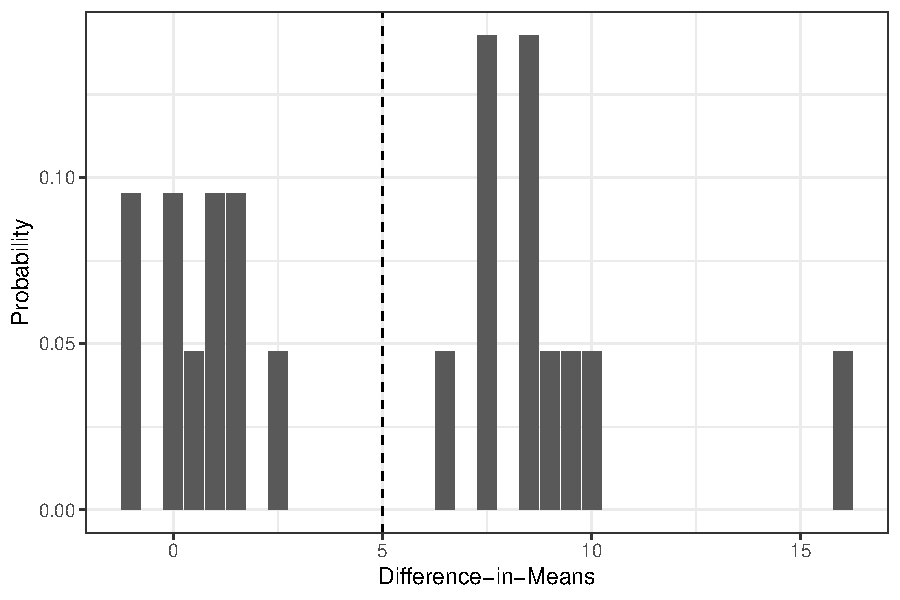
\includegraphics[width=0.9\linewidth]{cra_est_dist_plot.pdf}
\end{figure} 
\item What is the variance of this estimator?  
\item Why do we care about variance of an estimator?
\end{itemize}
\end{frame}
%------------------------------------------------------------------------
\begin{frame}
\frametitle{Variance of Difference-in-Means estimator} 
\begin{itemize}
\item Variance is average squared distance of estimator from its expected value:  
\begin{equation*}
\underbrace{\E\left[\underbrace{\left(\hat{\tau}\left(\bm{Z}, \bm{Y}\right) - \underbrace{\E\left[\hat{\tau}\left(\bm{Z}, \bm{Y}\right)\right]}_{\color{red}{\text{Expected value}}}\right)^2}_{\color{blue}{\text{Squared distance from expected value}}}\right]}_{\color{green}{\text{Average (or expected) squared distance}}}
\end{equation*} \pause
\item Diff-in-Means unbiased for $\tau$, so write variance as 
\begin{equation*}
\E\left[\left(\hat{\tau}\left(\bm{Z}, \bm{Y}\right) - \tau\right)^2\right]
\end{equation*} \pause
\item In ``village heads'' example with 21 possible assignments
\begin{align*}
\left(\hat{\tau}\left(\bm{z}_1, \bm{y}_1\right) - \tau\right)^2 \Pr\left(\bm{Z} = \bm{z}_1\right) + \ldots + \left(\hat{\tau}\left(\bm{z}_{21}, \bm{y}_{21}\right) - \tau\right)^2 \Pr\left(\bm{Z} = \bm{z}_{21}\right)
\end{align*}  
\item[] Variance is $\approx 21.19$
\end{itemize}
\end{frame}
%------------------------------------------------------------------------
\begin{frame}
\frametitle{Variance of Difference-in-Means estimator}
\begin{itemize}
\item Neyman (1923) derived expression for variance of Diff-in-Means under complete random assignment
\begin{equation*}
\Var\left[\hat{\tau}\left(\bm{Z}, \bm{Y}\right)\right] = \frac{1}{N - 1}\left(\frac{n_1 \mh{\sigma^2_{\bm{y}(\bm{0})}}}{n_0} + \frac{n_0 \mh{\sigma^2_{\bm{y}(\bm{1})}}}{n_1} + 2\mh{\sigma_{\bm{y}(\bm{0}), \bm{y}(\bm{1})}}\right)
\end{equation*}  
where 
\item[] $\sigma^2_{\bm{y}(\bm{0})} = \frac{1}{N} \sum \limits_{i = 1}^N \left(y_i(0) - \frac{1}{N} \sum \limits_{i = 1}^N y_i(0)\right)^2$ is var of control POs
\item[] $\sigma^2_{\bm{y}(\bm{1})} = \frac{1}{N} \sum \limits_{i = 1}^N \left(y_i(1) - \frac{1}{N} \sum \limits_{i = 1}^N y_i(1)\right)^2$ is var of treated POs
\item[] $\sigma_{\bm{y}(\bm{0}), \bm{y}(\bm{1})} = \frac{1}{N} \sum \limits_{i = 1}^N \left(y_i(0) - \frac{1}{N} \sum \limits_{i = 1}^N y_i(0)\right)\left(y_i(1) - \frac{1}{N} \sum \limits_{i = 1}^N y_i(1)\right)$ is cov of POs
\end{itemize} \pause
\vspace{1em}
$\star$ Note that $\mh{\sigma^2_{\bm{y}(\bm{0})}}$, $\mh{\sigma^2_{\bm{y}(\bm{1})}}$ and $\mh{\sigma_{\bm{y}(\bm{0}), \bm{y}(\bm{1})}}$ depend on unknown potential outcomes
\end{frame}
%------------------------------------------------------------------------
\begin{frame}
\frametitle{Variance of Difference-in-Means estimator}
\begin{itemize}
\item Sometimes you might see equivalent expression (Imbens and Rubin 2015)
\begin{equation*}
\dfrac{\mh{S_{\bm{y}(\bm{0})}}}{n_0} + \dfrac{\mh{S_{\bm{y}(\bm{1})}}}{n_1} - \dfrac{\mh{S_{\tau}}}{N},
\end{equation*}
where
\item[] $S_{\bm{y}(\bm{0})} = \frac{1}{N - 1} \sum \limits_{i = 1}^N \left(y_i(0) - \frac{1}{N} \sum \limits_{i = 1}^N y_i(0)\right)^2$
\item[] $S_{\bm{y}(\bm{1})} = \frac{1}{N - 1} \sum \limits_{i = 1}^N \left(y_i(1) - \frac{1}{N} \sum \limits_{i = 1}^N y_i(1)\right)^2$ 
\item[] $S_{\tau} = \frac{1}{N - 1} \sum \limits_{i = 1}^N \left(\tau_i - \frac{1}{N} \sum \limits_{i = 1}^N \tau_i\right)^2$
\end{itemize} \pause
\vspace{1em}
$\star$ Note that $\mh{S_{\bm{y}(\bm{0})}}$, $\mh{S_{\bm{y}(\bm{1})}}$ and $\mh{S_{\tau}}$ depend on unknown potential outcomes
\end{frame}
%------------------------------------------------------------------------
\begin{frame}
\frametitle{Variance of Difference-in-Means estimator}
\begin{itemize}
\item Example: ``Village heads'' study (Gerber and Green 2012, Chapter 2): \vspace{0.1in}
\item[]
\begin{center}
\begin{tabular}{l|rrr} \hline
& \multicolumn{3}{c}{Budget share (\%)} \\
Village &$\bm{\bm{y}(\bm{0})}$& $\bm{\bm{y}(\bm{1})}$& $\bm{\tau}$  \\ \hline
1& 10 & 15  & 5  \\
2& 15 & 15  & 0   \\ 
3& 20 & 30  & 10   \\
4& 20 & 15  & -5   \\
5& 10 & 20  & 10   \\
6& 15 & 15  & 0   \\
7& 15 & 30  & 15   \\ \hline
Average & 15 & 20 & 5  \\ \hline
\end{tabular}
\end{center} \vspace{0.5em} \pause
\item With access to true POs, we can directly calculate $\Var\left[\hat{\tau}\left(\bm{Z}, \bm{Y}\right)\right]$: \vspace{0.5em}
\item[] $\mh{\sigma^2_{\bm{y}(\bm{0})}} \approx 14.29$, $\mh{\sigma^2_{\bm{y}(\bm{1})}} \approx 42.86$, $\mh{\sigma_{\bm{y}(\bm{0}), \bm{y}(\bm{1})}} \approx 7.14$ \vspace{0.5em}
\item So, $\Var\left[\hat{\tau}\left(\bm{Z}, \bm{Y}\right)\right] = \frac{1}{N - 1}\bigg(\frac{n_1 \mh{\sigma^2_{\bm{y}(\bm{0})}}}{n_0} + \frac{n_0 \mh{\sigma^2_{\bm{y}(\bm{1})}}}{n_1} + 2\mh{\sigma_{\bm{y}(\bm{0}), \bm{y}(\bm{1})}}\bigg) \approx 21.19$ \pause \vspace{0.5em}
\item In practice, $\mh{\sigma^2_{\bm{y}(\bm{0})}}$, $\mh{\sigma^2_{\bm{y}(\bm{1})}}$ and $\mh{\sigma_{\bm{y}(\bm{0}), \bm{y}(\bm{1})}}$ unknown, so we estimate $\Var\left[\hat{\tau}\left(\bm{Z}, \bm{Y}\right)\right]$
\end{itemize}
\end{frame}
%------------------------------------------------------------------------
\section{Variance estimation}
\begin{frame}{Variance estimation} 
We showed that the Diference-in-Means estimator's variance is \vspace{1em}
\begin{equation*}
\Var\left[\hat{\tau}\left(\bm{Z}, \bm{Y}\right)\right] = \frac{1}{N - 1}\left(\frac{n_1 \bh{\sigma^2_{\bm{y}(\bm{0})}}}{n_0} + \frac{n_0 \bh{\sigma^2_{\bm{y}(\bm{1})}}}{n_1} + 2\mh{\sigma_{\bm{y}(\bm{0}), \bm{y}(\bm{1})}}\right)
\end{equation*}
\begin{itemize}
\item We have unbiased estimators for $\bh{\sigma^2_{\bm{y}(\bm{0})}}$ and $\bh{\sigma^2_{\bm{y}(\bm{1})}}$, but not $\mh{\sigma_{\bm{y}(\bm{0}), \bm{y}(\bm{1})}}$
\item So what do we do? \pause
\item We use \textbf{conservative} ``plug-in'' estimator (Neyman 1923)
\item \textbf{Conservative} means that
\begin{equation*}
\E\left[\widehat{\Var}\left[\hat{\tau}\left(\bm{Z}, \bm{Y}\right)\right]\right] \geq \Var\left[\hat{\tau}\left(\bm{Z}, \bm{Y}\right)\right]
\end{equation*} \pause
\item When potential outcomes perfectly positively correlated
\begin{equation*}
\E\left[\widehat{\Var}\left[\hat{\tau}\left(\bm{Z}, \bm{Y}\right)\right]\right] = \Var\left[\hat{\tau}\left(\bm{Z}, \bm{Y}\right)\right]
\end{equation*}
\item Otherwise, $\widehat{\Var}\left[\hat{\tau}\left(\bm{Z}, \bm{Y}\right)\right]$ is positively biased (conservative) \pause
\item Potential outcomes will be perfectly positively correlated if and only if \\ $\tau_i$ is the same for all $i = 1, \ldots , N$ units
\end{itemize}
\end{frame}
%------------------------------------------------------------------------
\begin{frame}{Conservative variance estimator} 
\begin{equation*}
\Var\left[\hat{\tau}\left(\bm{Z}, \bm{Y}\right)\right] = \frac{1}{N - 1}\left(\frac{n_1 \bh{\sigma^2_{\bm{y}(\bm{0})}}}{n_0} + \frac{n_0 \bh{\sigma^2_{\bm{y}(\bm{1})}}}{n_1} + 2\mh{\sigma_{\bm{y}(\bm{0}), \bm{y}(\bm{1})}}\right)
\end{equation*} \pause
\begin{itemize}
\item The maximum possible value of $2\mh{\sigma_{\bm{y}(\bm{0}), \bm{y}(\bm{1})}}$ is $\bh{\sigma^2_{\bm{y}(\bm{0})}} + \bh{\sigma^2_{\bm{y}(\bm{1})}}$ 
\item So substitute $\bh{\sigma^2_{\bm{y}(\bm{0})}} + \bh{\sigma^2_{\bm{y}(\bm{1})}}$ for $2\mh{\sigma_{\bm{y}(\bm{0}), \bm{y}(\bm{1})}}$: \pause
\begin{align*}
\Var\left[\hat{\tau}\left(\bm{Z}, \bm{Y}\right)\right] & = \frac{1}{N - 1}\left(\frac{n_1 \bh{\sigma^2_{\bm{y}(\bm{0})}}}{n_0} + \frac{n_0 \bh{\sigma^2_{\bm{y}(\bm{1})}}}{n_1} + \left(\bh{\sigma^2_{\bm{y}(\bm{0})}} + \bh{\sigma^2_{\bm{y}(\bm{1})}}\right)\right) \\
& = \frac{N}{N - 1}\left(\frac{\bh{\sigma^2_{\bm{y}(\bm{0})}}}{n_0} + \frac{\bh{\sigma^2_{\bm{y}(\bm{1})}}}{n_1}\right)
\end{align*} \pause
\item Now all quantities can be estimated! \pause
\item So, just ``plug-in'' estimators $\hat{\sigma}^2_{\bm{y}(\bm{0})}$ and $\hat{\sigma}^2_{\bm{y}(\bm{1})}$ for $\bh{\sigma^2_{\bm{y}(\bm{0})}}$ and $\bh{\sigma^2_{\bm{y}(\bm{1})}}$
\begin{equation}
\widehat{\Var}\left[\hat{\tau}\left(\bm{Z}, \bm{Y}\right)\right] = \frac{N}{N - 1}\left(\frac{\hat{\sigma}^2_{\bm{y}(\bm{0})}}{n_0} + \frac{\hat{\sigma}^2_{\bm{y}(\bm{1})}}{n_1} \right)
\end{equation}
\item For exact expressions of $\hat{\sigma}^2_{\bm{y}(\bm{0})}$ and $\hat{\sigma}^2_{\bm{y}(\bm{1})}$, see \hyperlink{Variance estimators}{\beamerbutton{Variance estimators}}
\end{itemize}
\end{frame}
%------------------------------------------------------------------------
\begin{frame}{Variance estimation} 
\vfill
\begin{itemize} \vfill
\item Here is the conservative variance estimator in ``village heads'' example: \vfill
\begin{figure}[H]
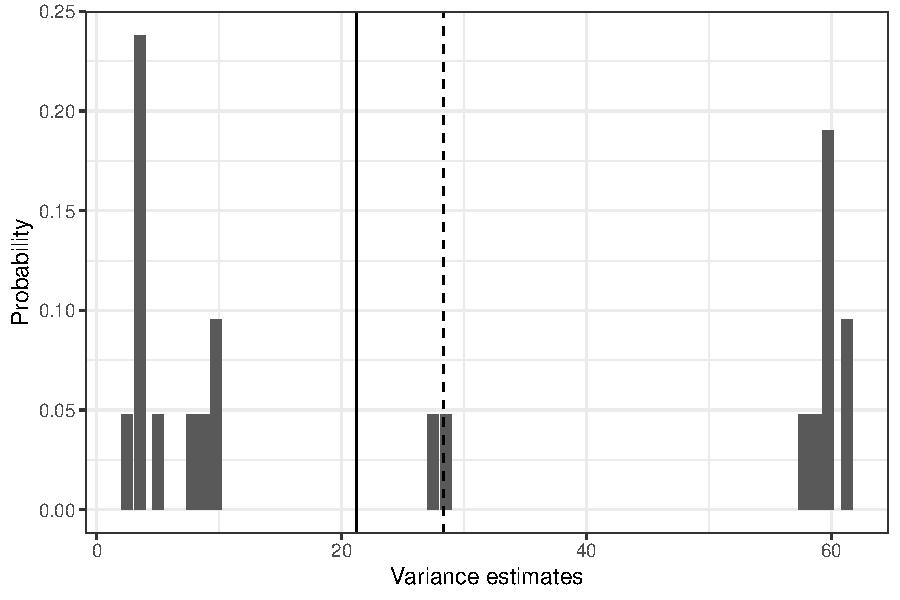
\includegraphics[width=0.8\linewidth]{cra_var_est_dist_plot.pdf}
\end{figure} \vfill
\item[] \small \textbf{Solid} line is true variance of Difference-in-Means estimator, $\Var\left[\hat{\tau}\left(\bm{Z}, \bm{Y}\right)\right]$  \vfill
\item[] \textbf{Dashed} line is expected value of conservative estimator, $\E\left[\widehat{\Var}\left[\hat{\tau}\left(\bm{Z}, \bm{Y}\right)\right]\right]$ \normalsize \vfill
\end{itemize} \vfill
\end{frame}
%------------------------------------------------------------------------
\section{Asymptotic properties}
\begin{frame}{Asymptotics}
\vfill
\begin{itemize} \vfill
\item So far, we have derived\vfill
\begin{enumerate} \vfill
\item unbiased Difference-in-Means estimator of ATE \vfill
\item variance of Difference-in-Means estimator \vfill
\item conservative estimator of Difference-in-Means estimator's variance
\vfill\end{enumerate} \vfill \pause
\item All of these derivations were for a fixed $N$, either small or large \vfill
\item Now let's see what happens to our estimator when $N$ grows large, $N \to \infty$ \vfill
\item But first, why do we care? \pause \vfill
\item[] $N$ never goes to $\infty$ in an actual experiment \vfill
\item[] But properties as $N \to \infty$ \textbf{approximate} properties with fixed, but large $N$ \vfill
\end{itemize} \vfill
\end{frame}
%------------------------------------------------------------------------
\section{Consistent estimation}
\begin{frame}{Consistent estimation}
\vfill
\begin{itemize} \vfill
\item Difference-in-Means estimator is consistent: \pause \vfill
\begin{equation*}
\lim \limits_{N \to \infty} \Pr\left(\left\lvert \hat{\tau}\left(\bm{Z}, \bm{Y}\right) - \tau \right\rvert < \epsilon \right) = 1 \text{ for all } \epsilon > 0
\end{equation*} \pause \vfill
\item In words: \vfill
\begin{center}
Pick any $\epsilon$ you want, no matter how small. There will be some value $N^{*}$ such that, if size of experiment is greater than $N^*$, 
the probability of an estimate within a distance of $\epsilon$ from the truth is equal to $1$.
\end{center} \pause \vfill
\item Intuitively, with large experiment, our estimate will be close to true ATE! \vfill
\end{itemize}
\vfill
\end{frame}
%------------------------------------------------------------------------
\begin{frame}{Consistent estimation}
\vfill
\begin{itemize} \vfill
\item ``Village heads'' example: \vfill
\begin{figure}[H]
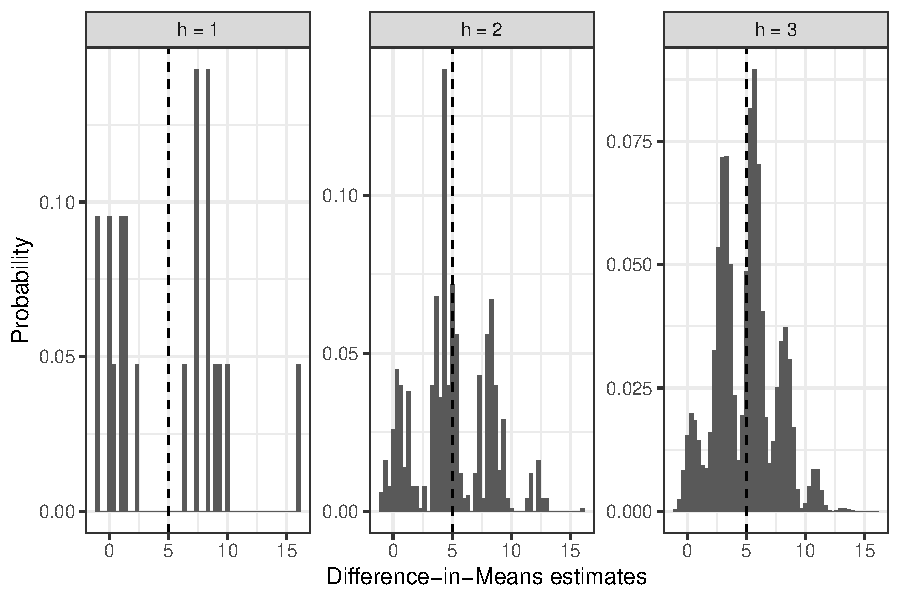
\includegraphics[width=\linewidth]{asymp_ests_plot.pdf}
\end{figure}
\end{itemize}
\vfill
\end{frame}
%------------------------------------------------------------------------
\section{Hypothesis testing}
\begin{frame}{Hypothesis tests of the weak null}
\begin{itemize}
\item The finite population CLT tells us that 
\begin{align*}
\cfrac{\hat{\tau}\left(\bm{Z}, \bm{Y}\right) - \E\left[\hat{\tau}\left(\bm{Z}, \bm{Y}\right)\right]}{\sqrt{\Var\left[\hat{\tau}\left(\bm{Z}, \bm{Y}\right)\right]}} & \overset{d}{\to} \mathcal{N}\left(0, 1\right)
\end{align*}  \pause 
\item Diff-in-Means is unbiased, so write
\begin{align*}
\cfrac{\hat{\tau}\left(\bm{Z}, \bm{Y}\right) - \tau}{\sqrt{\Var\left[\hat{\tau}\left(\bm{Z}, \bm{Y}\right)\right]}} & \overset{d}{\to} \mathcal{N}\left(0, 1\right)
\end{align*} \pause
\item The CLT is an asymptotic results as $N \to \infty$
\item But we can bound error of Normal approximation for fixed $N$ \pause
\item Thus, with experiments of at least moderate size and outcomes that aren't too skewed or have extreme outliers,
\begin{align*}
\cfrac{\hat{\tau}\left(\bm{Z}, \bm{Y}\right) - \tau}{\sqrt{\Var\left[\hat{\tau}\left(\bm{Z}, \bm{Y}\right)\right]}} & \overset{\text{approx.}}{\sim} \mathcal{N}\left(0, 1\right)
\end{align*} \pause
\item This justifies use of standard Normal distribution for hypothesis tests
\end{itemize}
\end{frame}
%------------------------------------------------------------------------
\begin{frame}{Hypothesis tests of the weak null}
\vfill
\begin{itemize} \vfill
\item ``Village heads'' example: \vfill
\begin{figure}[H]
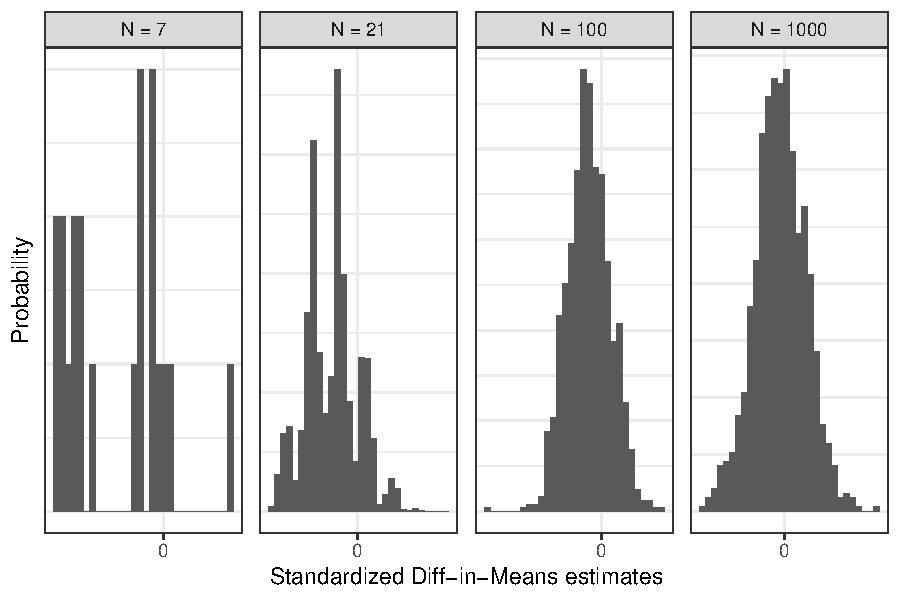
\includegraphics[width=\linewidth]{asymp_stand_ests_plot.pdf}
\end{figure}
\end{itemize}
\vfill
\end{frame}
%------------------------------------------------------------------------
\begin{frame}{Hypothesis tests of the weak null}
\begin{itemize}
\item To test null hypothesis relative to alternative
\begin{align*}
H_0: & \tau = \tau_0 \text{ versus either } \\
H_A: & \tau > \tau_0, \, H_A: \tau < \tau_0 \text{ or } H_A: \left\lvert \tau \right\rvert > \left\lvert \tau_0 \right \rvert
\end{align*} \pause
\item Calculate upper(u), lower(l) or two-sided(t) p-value as 
\begin{align*}
p_u & =  1 - \Phi\left(\frac{\hat{\tau}\left(\bm{Z}, \bm{Y}\right) - \tau_0}{\sqrt{\widehat{\Var}\left[\hat{\tau}\left(\bm{Z}, \bm{Y}\right)\right]}}\right) \\
p_l & =  \Phi\left(\frac{\hat{\tau}\left(\bm{Z}, \bm{Y}\right) - \tau_0}{\sqrt{\widehat{\Var}\left[\hat{\tau}\left(\bm{Z}, \bm{Y}\right)\right]}}\right) \\
p_t & = 2\left(1 - \Phi\left(\frac{\left\lvert\hat{\tau}\left(\bm{Z}, \bm{Y}\right) - \tau_0\right\rvert}{\sqrt{\widehat{\Var}\left[\hat{\tau}\left(\bm{Z}, \bm{Y}\right)\right]}}\right)\right)
\end{align*} \pause
\item If p-value is less than size $\alpha$-level of test, reject. Otherwise, don't
\item Note that, since we don't know $\Var\left[\hat{\tau}\left(\bm{Z}, \bm{Y}\right)\right]$, \\ we have used its conservative estimator instead, $\widehat{\Var}\left[\hat{\tau}\left(\bm{Z}, \bm{Y}\right)\right]$
\end{itemize}
\end{frame}
%------------------------------------------------------------------------
\begin{frame}{Hypothesis tests of the weak null}
\bh{Hypothesis tests susceptible to two errors}:
\begin{itemize}
\item Type I error: Rejecting null hypothesis when it is true
\item Type II error: \textit{Failing} to reject null hypothesis when it is false
\end{itemize} \pause 
\bh{A good test} controls these errors:
\begin{enumerate}
\item Type I error probability is less than or equal to size ($\alpha$-level) of test
\item Power (1 - type II error probability) is at least as great as $\alpha$-level
\item Power tends to $1$ as $N \to \infty$
\end{enumerate}  
\end{frame}
%------------------------------------------------------------------------
\begin{frame}{Hypothesis tests of the weak null}
\vfill
\begin{itemize} \vfill
\item We can prove that tests of weak null satisfy (1) -- (3) as $N \to \infty$ \vfill 
\item Thus, when experiments are large, we can often safely use such tests \vfill
\item But (1) -- (3) may not always be satisfied when experiments are small, have skewed outcome distributions or extreme outliers \vfill
\end{itemize}
\end{frame}
%------------------------------------------------------------------------
\begin{frame}{Confidence intervals}
\vfill
\begin{itemize} \vfill
\item Equivalence between hypothesis testing and confidence intervals
\item Confidence interval is set of null hypotheses we fail to reject
\end{itemize}
Consider two-sided confidence interval, $\mathcal{C}_t$:
\footnotesize
\begin{equation*}
\begin{split}
\mathcal{C}_t & = \left\{\tau_0 : \left\lvert \cfrac{\hat{\tau}\left(\bm{Z}, \bm{Y}\right)- \tau_0}{\sqrt{\widehat{\Var}\left[\hat{\tau}\left(\bm{Z}, \bm{Y}\right)\right]}} \right\rvert \leq z_{1 - \alpha/2}\right\} \\ 
& = \left\{\tau_0 : - z_{1 - \alpha/2} \leq \cfrac{\hat{\tau}\left(\bm{Z}, \bm{Y}\right)- \tau_0}{\sqrt{\widehat{\Var}\left[\hat{\tau}\left(\bm{Z}, \bm{Y}\right)\right]}} \leq z_{1 - \alpha/2} \right\} \\ 
& = \left\{\tau_0 : - z_{1 - \alpha/2} \sqrt{\widehat{\Var}\left[\hat{\tau}\left(\bm{Z}, \bm{Y}\right)\right] }\leq \hat{\tau}\left(\bm{Z}, \bm{Y}\right)- \tau_0 \leq z_{1 - \alpha/2} \sqrt{\widehat{\Var}\left[\hat{\tau}\left(\bm{Z}, \bm{Y}\right)\right] }\right\} \\ 
& = \left\{\tau_0 : -\hat{\tau}\left(\bm{Z}, \bm{Y}\right)- z_{1 - \alpha/2} \sqrt{\widehat{\Var}\left[\hat{\tau}\left(\bm{Z}, \bm{Y}\right)\right] }\leq - \tau_0 \leq - \hat{\tau}\left(\bm{Z}, \bm{Y}\right)+ z_{1 - \alpha/2} \sqrt{\widehat{\Var}\left[\hat{\tau}\left(\bm{Z}, \bm{Y}\right)\right] }\right\} \\ 
& = \left\{\tau_0 : \hat{\tau}\left(\bm{Z}, \bm{Y}\right)+ z_{1 - \alpha/2} \sqrt{\widehat{\Var}\left[\hat{\tau}\left(\bm{Z}, \bm{Y}\right)\right] }\geq \tau_0 \geq  \hat{\tau}\left(\bm{Z}, \bm{Y}\right)- z_{1 - \alpha/2} \sqrt{\widehat{\Var}\left[\hat{\tau}\left(\bm{Z}, \bm{Y}\right)\right] }\right\} \\ 
& = \left\{\tau_0 : \hat{\tau}\left(\bm{Z}, \bm{Y}\right)- z_{1 - \alpha/2} \sqrt{\widehat{\Var}\left[\hat{\tau}\left(\bm{Z}, \bm{Y}\right)\right] }\leq \tau_0 \leq \hat{\tau}\left(\bm{Z}, \bm{Y}\right)+ z_{1 - \alpha/2} \sqrt{\widehat{\Var}\left[\hat{\tau}\left(\bm{Z}, \bm{Y}\right)\right] }\right\}
\end{split}
\end{equation*}
\normalsize
\end{frame}
%------------------------------------------------------------------------


\begin{frame}[t, label = Variance estimators]
\frametitle{Appendix: Estimator of Difference-in-Means estimator's variance}
\vfill
Neyman's conservative estimator of the Difference-in-Means estimator's variance is 
\begin{equation*}
\widehat{\Var}\left[\hat{\tau}\left(\bm{Z}, \bm{Y}\right)\right] = \frac{N}{N - 1}\left(\frac{\hat{\sigma}^2_{\bm{y}(\bm{0})}}{n_0} + \frac{\hat{\sigma}^2_{\bm{y}(\bm{1})}}{n_1} \right),
\end{equation*}
where 
\begin{align*}
\hat{\sigma}^2_{\bm{y}(\bm{0})} & = \left(\frac{N - 1}{N\left(n_0 - 1\right)}\right)\sum \limits_{i: Z_i = 0}^N \left(y_i(0) - \hat{\mu}_{\bm{y}(\bm{0})}\right)^2 \\
\hat{\sigma}^2_{\bm{y}(\bm{1})} & = \left(\frac{N - 1}{N\left(n_1 - 1\right)}\right)\sum \limits_{i: Z_i = 1}^{n} \left(y_i(1) - \hat{\mu}_{\bm{y}(\bm{1})}\right)^2 \\ 
\hat{\mu}_{\bm{y}(\bm{0})} & = \left(\frac{1}{n_0}\right) \sum \limits_{i = 1}^N \left(1 - Z_i\right)y_i(0) \\ 
\hat{\mu}_{\bm{y}(\bm{1})} & = \left(\frac{1}{n_1}\right) Z_i y_i(1)
\end{align*}
\vfill
\end{frame}
\end{document}